%%%%%%%%%%%%%%%%%%%%%%%%%%%%%%%%%%%%%%%%%%%%%%%%%%%%%%%%%%%%%%%%%%%%
% This is a thesis template for Gebze Technical University.
%
% Please only edit the areas proceeded by a comment starting with %%
% otherwise the template may be broken.
%
% This file is only to be used for editing the general fields
% and inputting the body of the thesis in the designated areas.
% Please write the body of the thesis in separate files, and input
% them as shown in the comment preceding the area.
%
% Created in Aug 2021 by Usama Derbashi.
%%%%%%%%%%%%%%%%%%%%%%%%%%%%%%%%%%%%%%%%%%%%%%%%%%%%%%%%%%%%%%%%%%%%
\documentclass[12pt]{report}


% Language and typeset setting
\usepackage[english]{babel}
\usepackage[a4paper,top=25mm,bottom=25mm,left=40mm,right=25mm]{geometry}
\usepackage[onehalfspacing]{setspace}
\usepackage{algorithm, algpseudocode}
\usepackage{indentfirst}
\usepackage{multirow}
\usepackage[justification=centering]{caption}
\usepackage{pdflscape}
\usepackage{tikz}
\usetikzlibrary{shapes.geometric, arrows}

\tikzstyle{actor} = [draw, ellipse, minimum width=3cm, minimum height=1cm, text centered, draw=black, fill=red!30]
\tikzstyle{usecase} = [ellipse, draw=blue, fill=blue!20, text centered, minimum width=3cm, minimum height=1cm, text width=2.5cm]



\setlength{\parindent}{1cm}
\setlength{\abovecaptionskip}{12pt plus 0pt minus 0pt}
\setlength{\belowcaptionskip}{12pt plus 0pt minus 0pt}
\setlength{\textfloatsep}{18.0pt plus 0.0pt minus 0.0pt}
\setlength{\floatsep}{18.0pt plus 0.0pt minus 0.0pt}
\setlength{\intextsep}{18.0pt plus 0.0pt minus 0.0pt}
\setlength{\skip\footins}{18.0pt plus 0.0pt minus 0.0pt}

% Core packages and settings
\usepackage[colorlinks=false]{hyperref}
\usepackage{amsmath}

\usepackage{titlesec} %setting the titles of chapters and sections
\setcounter{secnumdepth}{4}
\setcounter{tocdepth}{4}
\titleformat{\chapter}[hang]{\normalfont\bfseries\MakeUppercase}{}{0pt}{\LARGE\thechapter. }
\titleformat{\section}[hang]{\normalfont\bfseries}{}{0pt}{\Large\thesection. }
\titleformat{\subsection}[hang]{\normalfont\bfseries}{}{0pt}{\large\thesubsection. }
\titleformat{\subsubsection}[hang]{\normalfont\bfseries}{}{0pt}{\large\thesubsubsection. }
\titlespacing*{\chapter}{0pt}{0pt}{18pt}
\titlespacing*{\section}{0pt}{18pt}{18pt}
\titlespacing*{\subsection}{0pt}{18pt}{18pt}
\titlespacing*{\subsubsection}{0pt}{18pt}{18pt}

\usepackage{graphicx}
\graphicspath{{./Imgs/}} %pointing the directory of images

\usepackage{fancyhdr} % setting footers
\usepackage{etoolbox} 
\renewcommand{\headrulewidth}{0pt}
\patchcmd{\chapter}{\thispagestyle{plain}}{\thispagestyle{fancy}}{}{}
\pagestyle{fancy}
\fancyhf{}
\fancyfoot[C]{\fontsize{11pt}{11pt}\thepage}

\usepackage[style=ieee]{biblatex}
\addbibresource{refs.bib}
\usepackage{csquotes}% Needed for babel(in biblatex)

\usepackage[bottom, perpage]{footmisc}%% amkes footnotes at the bottom

\usepackage{GTUThesis}


% Additional packages if needed
%% For the sake of not messing the template add them here
\usepackage{lipsum}

\usepackage{tikz}
\usetikzlibrary{shapes.geometric, arrows}

\tikzstyle{actor} = [draw, ellipse, minimum width=3cm, minimum height=1cm, text centered, draw=black, fill=red!30]
\tikzstyle{usecase} = [ellipse, draw=blue, fill=blue!20, text centered, minimum width=3cm, minimum height=1cm, text width=2cm]


% Important information
%% Make sure to enter all the info below
\title{AR Based Quality Control System On VisionPro (Phase 2)}
\author{
    BİLAL GÖKÇE 
	\linebreak
    MELİKE SEYİTOĞLU
}
\faculty{Faculty of Engineering}
\department{Computer Engineering Department}
\supervisor{Doç. Dr. Yakup GENÇ}
\theyear{2025}


\begin{document}

%Front Matter
\pagenumbering{roman} %start with roman numbering 
\projecttitlepageenglish
\maketitle
\setcounter{page}{3} %the first two title pages are not counted so this is a buffer
\begin{outertitles} % makes titles centred

%% below enter as follows 
%% {DATE_OF_DEMO}{JURY}
%% Note that JURY should be comma separated
\makejury{../../2025}{Dr. Salih SARP}

\chapter*{Abstract}
\addcontentsline{toc}{chapter}{Abstract}

%% Edit below this line

This thesis presents the design and implementation of an augmented reality (AR) quality control system tailored for the Apple Vision Pro. Building upon prior work in tablet-based AR inspection, this project leverages the Vision Pro’s advanced spatial tracking, gesture-based interaction, and powerful hardware to deliver a more immersive and precise quality control experience.

The system introduces new capabilities, including real-time object tracking, dynamic custom annotation functionality, and improved reporting features. Testing shows that the system achieves robust tracking stability, efficient annotation search, and inspection workflows with completion times close to those of leading tablet-based solutions.

While some limitations persist—such as input method latency and restrictions inherent to the Apple development environment—the results indicate that the Vision Pro is well-suited for complex industrial quality control tasks. The thesis concludes with recommendations for future development, such as automated inspection point generation and support for richer annotation types. Overall, this work demonstrates the strong potential of next-generation AR platforms to modernize and improve industrial inspection processes.

%% Until here
\vfill
%% Edit after {Keywords:}
\textbf{Keywords:} AVP, UI/UX, AR.
\clearpage
\chapter*{Acknowledgement}
\addcontentsline{toc}{chapter}{Acknowledgement}

We would like to express our deepest gratitude to our advisor, Dr. Yakup GENÇ, for his support in providing us access to the Apple Vision Pro and related devices, as well as the invaluable opportunities that have greatly contributed to the success of this project.

We also thank our classmates Onur Atasever and Ahmet Hamza Şiyak for their kind assistance in lending their iPhone Pro devices, which was essential for object capture and model generation during the project.

\vspace{1cm}
\begin{flushright}
    BİLAL GÖKÇE \\
    MELİKE SEYİTOĞLU \\
\end{flushright}
\begin{flushleft}
    June, 2025
\end{flushleft}
\clearpage
\chapter*{List of Symbols and Abbreviations}
\addcontentsline{toc}{chapter}{List of Symbols and Abbreviations}

\begin{tabular}{lcl}
    \textbf{Symbol or}&&\\
    \textbf{Abbreviation} &:& \textbf{Explanation}\\
    AR &:& Augmented Reality\\
    AVP &:& Apple Vision Pro\\
    ARKit &:& Apple's Augmented Reality Framework\\
    UI &:& User Interface\\
    UX &:& User Experience\\
    USDZ &:& Universal Scene Description (3D File Format)\\
    libxlsxwriter &:& A C library for creating Excel files\\
    FPS &:& Frames Per Second\\
    ms &:& Milliseconds\\
    $t_{avg}$ &:& Average Latency\\
    ML &:& Machine Learning\\
    LLM &:& Large Language Model\\
    CAD &:& Computer-Aided Design\\
    SceneKit &:& Apple’s 3D Graphics Framework\\
    GPU &:& Graphics Processing Unit\\
    SiriKit &:& Apple’s Voice Interaction Framework\\
    LiDAR &:& Light Detection and Ranging (3D scanning sensor)\\
    Object Capture &:& Photogrammetry-based 3D reconstruction process\\
\end{tabular}

\clearpage


\tableofcontents
\addcontentsline{toc}{chapter}{Contents}
\clearpage

\listoffigures
\addcontentsline{toc}{chapter}{List of Figures}
\clearpage

\listoftables
\addcontentsline{toc}{chapter}{List of Tables}
\clearpage



\end{outertitles}
\fancyhf{}%reset footer
\fancyfoot[R]{\fontsize{11pt}{11pt}\thepage}%page numbers in the corner
\addtocontents{toc}{\protect\vspace{18pt}}
\pagenumbering{arabic}%turn to arabic numbers

% Mainmatter

%% Only input files, don't write here
%% \input{./Body/Mainmatter/FILE}
\chapter{Introduction}

Augmented reality (AR) technologies have revolutionized various industries, offering innovative solutions to complex problems. Quality control systems are one such area where AR can provide immense value. While similar applications exist on platforms like the iPad, their limitations in spatial capabilities and less intuitive interaction methods make them less suitable for high-precision tasks. In this project, we have developed a quality control system tailored for the Apple Vision Pro (AVP), leveraging its advanced spatial capabilities, immersive experience, and intuitive gesture-based controls.

Having completed the core functionality in the first phase—including inspection workflows, basic positioning, and automated report generation—this second phase of our project shifts focus to advancing object tracking and introducing custom annotation features. These enhancements aim to make the system more dynamic and adaptable, harnessing the Vision Pro’s superior sensor and processing capabilities. By leveraging this more powerful hardware, we expect to achieve greater tracking precision and provide a richer, more intuitive user experience for industrial quality control applications.

\section{Project Definition}

The aim of this project is to develop a quality control system specifically designed for the Apple Vision Pro (AVP). Unlike iPads, which have limited spatial features, the AVP offers advanced spatial capabilities and immersive interaction methods that make it ideal for high-precision tasks. This system leverages the AVP’s strengths to improve accuracy and efficiency in quality control processes.

The key functionalities include aligning 3D CAD models with real-world objects, enabling interactive inspections at both predefined and custom annotation points, supporting dynamic (user-defined) annotations, implementing real-time object tracking (not just initial positioning), and generating detailed quality analysis reports. Unlike tablet-based systems—which often suffer from limited depth perception, reduced tracking stability, and less natural interaction methods—our solution leverages Vision Pro’s advanced hardware to overcome these barriers. By providing enhanced spatial understanding, intuitive gesture and gaze-based controls, and robust tracking, this project offers a precise, efficient, and user-friendly platform for industrial quality control applications.


% This project focuses on designing and implementing a quality control system for the Apple Vision Pro (AVP). The system utilizes the AVP's cutting-edge spatial and interaction capabilities to enhance accuracy and user experience. The core functionality revolves around:
% \begin{itemize}
%     \item Aligning 3D CAD models with real-world objects to identify differences.
%     \item Providing users with tools for interactive and natural inspection using gesture-based controls.
%     \item Generating quality analysis reports in Excel format for documentation and review.
%     \item Allowing users to inspect predefined points on models for detailed quality control.
% \end{itemize}

% During the inspection process, users can select specific inspection points on the model to perform quality checks. These inspections can include:
% \begin{itemize}
%     \item Yes/No Verification: Confirming whether a feature meets the required specifications.
%     \item Description-based Analysis: Providing detailed notes about the inspected feature.
%     \item Count-based Evaluation: Counting the number of specific elements.
% \end{itemize}

% The application is designed to support industries where precise quality control is critical, such as manufacturing, automotive, and aerospace.

\section{Project Aims}

The primary aims of the second phase of this project are as follows:
\begin{enumerate}
    \item \textbf{Enhanced User Experience:} Refine and optimize the UI/UX for even more intuitive, gesture-driven interaction, leveraging advanced features like gaze tracking and improved finger gesture recognition.
    \item \textbf{Precise Object Tracking:} Move beyond initial alignment to implement robust, real-time tracking of objects in the environment, enabling consistent spatial registration and minimizing drift during use.
    \item \textbf{Custom Annotations:} Enable users to create, place, and edit dynamic, user-defined annotation points directly in AR, rather than being limited to only predefined inspection locations.
    \item \textbf{Advanced Reporting:} Extend the reporting functionality to include annotation data, allowing users to generate comprehensive quality control reports that reflect both inspection results and user-added insights.
    \item \textbf{Performance Improvements:} Further optimize system performance to ensure smooth, low-latency operation—even with the added complexity of dynamic annotations and continuous tracking.
\end{enumerate}

These enhancements build directly upon the foundation established in the first phase, aiming to deliver a more dynamic, precise, and adaptable quality control solution powered by the Apple Vision Pro.
\chapter{Project Details}

This chapter provides an in-depth explanation of the project's components and tools used. The system was developed using Swift, Xcode, RealityComposer Pro and the Object Capture app to leverage the capabilities of Apple Vision Pro.

% \section{UI/UX Design}
\section{UI/UX Design}
The application has a streamlined user interface with a single window navigating between different views to ensure an intuitive and user-friendly experience. Below is the flow of UI/UX interactions. Some parts of the interface were designed and implemented during the first semester. In the second semester, we expanded the system by integrating object tracking and annotation.

In addition to these modifications, button visuals were revised to provide a more professional appearance. (Figures \ref{fig:button_before} and \ref{fig:button_after} show the button appearance before and after the updates.)

\begin{figure}[h!]
    \centering
    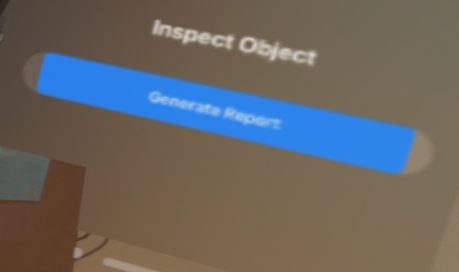
\includegraphics[width=0.4\textwidth]{button_before.png}
    \caption{\centering Button appearance before visual update.}
    \label{fig:button_before}
\end{figure}

\begin{figure}[h!]
    \centering
    
\includegraphics[width=0.4\textwidth]{button_after.png}
    \caption{\centering Button appearance after visual update.}
    \label{fig:button_after}
\end{figure}

\subsection{Initial Session Start}
The application starts with a view prompting the user to begin an ARKit session. In the first semester, this session was primarily responsible for initializing plane detection and world tracking. In the current version, it also starts object tracking for all referenced objects. The interface provides visual indicators to guide the user during this setup phase. (Figure \ref{fig:ui_session_start} shows the UI at this stage.)
\begin{figure}[H]
    \centering
    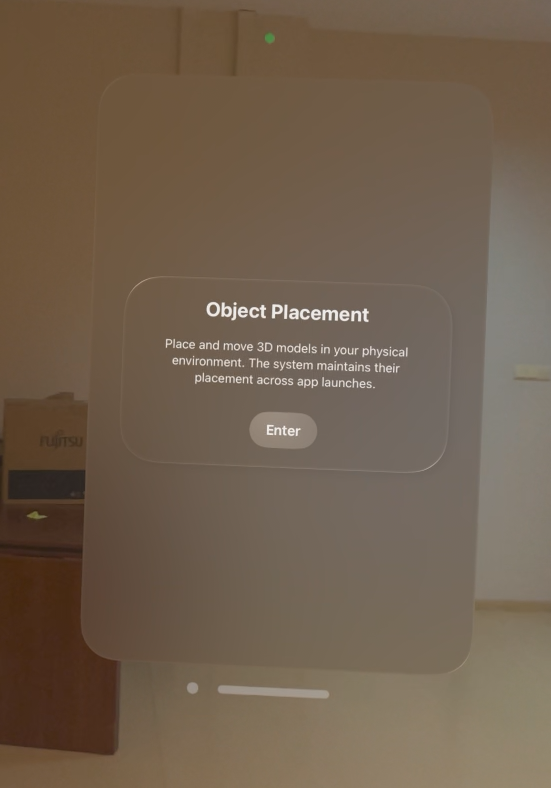
\includegraphics[width=0.37\textwidth]{session_start_ui.png} % Replace with your image file name
    \caption{UI for starting the ARKit session.}
    \label{fig:ui_session_start}
\end{figure}

\subsection{Object Selection Menu}
After initializing the session, the user is directed to an object selection menu. In this view:
\begin{itemize}
    \item The user selects an object from the available options.
    \item When an object is clicked, the \texttt{selectedObject} state is updated.
    \item The selected object is prepared for placement. (Figure \ref{fig:ui_object_selection} shows the object selection menu.)
\end{itemize}

While the basic selection mechanism was implemented in the first semester, this semester we expanded the menu by adding new models specifically designed to demonstrate the object tracking feature. Each of these new models is associated with a reference object file used for object recognition, along with a corresponding USDZ format 3D model for rendering in AR.

\begin{figure}[h!]
    \centering
    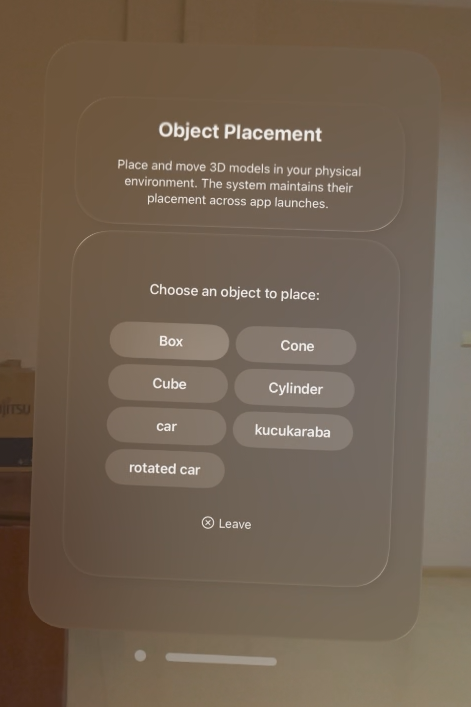
\includegraphics[width=0.4\textwidth]{object_selection_ui.png} % Replace with your image file
    \caption{Object selection menu UI.}
    \label{fig:ui_object_selection}
\end{figure}

\subsection{Initial Object Placement}
This component was implemented during the first semester and remains unchanged in the current version. During the initial placement of the selected object:
\begin{itemize}
    \item Placement tooltips are displayed to guide the user on positioning the object accurately.
    \item Visual aids ensure the user understands how to interact with the AR environment. (Figure \ref{fig:ui_initial_placement} shows the placement tooltip.)
\end{itemize}
\begin{figure}[H]
    \centering
    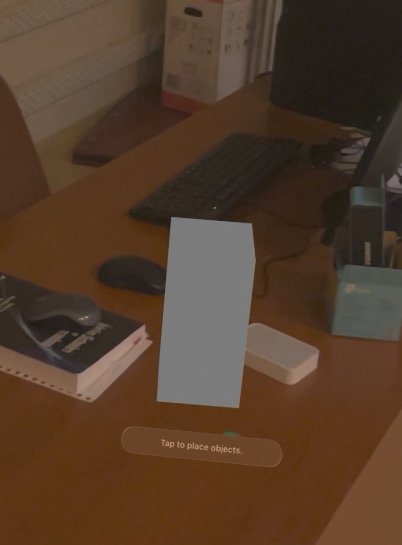
\includegraphics[width=0.4\textwidth]{object_placement_tooltips.png} % Replace with your image file
    \caption{Placement tooltips during initial object placement.}
    \label{fig:ui_initial_placement}
\end{figure}

\subsection{Object Interaction View}
If there is already a placed object, the application navigates directly to the object interaction view. This view was initially developed in the first semester to support repositioning, inspection, and removal of the placed object. In the second semester, this view was extended with additional functionality, including a new annotation interaction feature and the relocation of the \textit{Generate Report} button.

\begin{itemize}
    \item The user can perform repositioning, inspection, annotation, report generation, or removal of the placed object. The interface displays buttons for these actions, as shown in Figure \ref{fig:object_interaction_view}.
\end{itemize}

\begin{figure}[H]
    \centering
    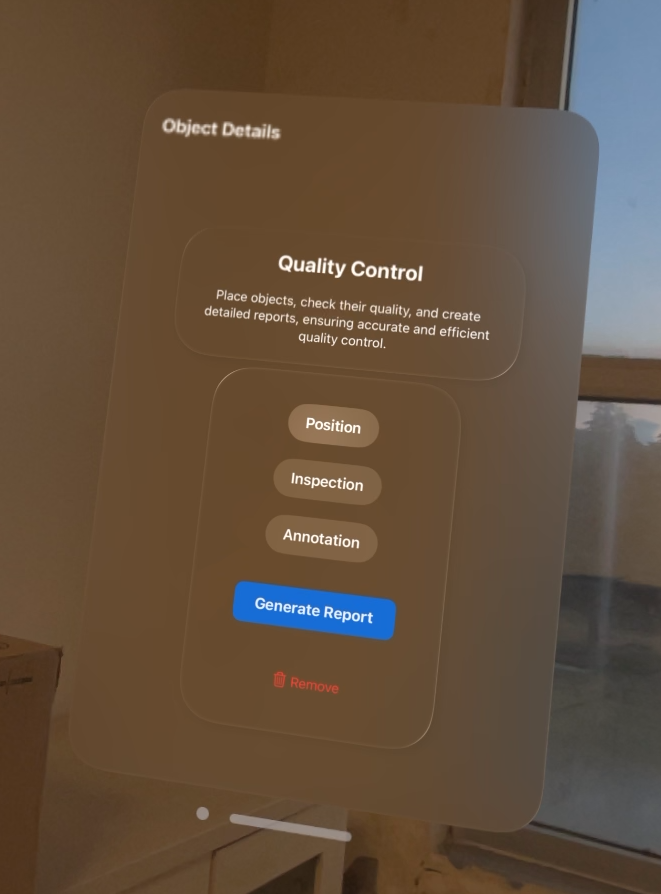
\includegraphics[width=0.39\textwidth]{object_interaction_view.png}
    \caption{\centering UI showing the buttons for repositioning, inspection, annotation, report generation, and removal.}
    \label{fig:object_interaction_view}
\end{figure}


\begin{itemize}
    \item Action buttons allow the user to activate the following functionalities:
    \begin{itemize}

        \item \textbf{Repositioning:} Includes rotation, left/right movement, and forward/backward movement. The user can use pinch and drag gestures (thumb and index finger) to perform the action. Only one action can be performed at a time.

        In addition to these basic controls, we introduced new buttons in the second semester to support object tracking visualization:
        \begin{itemize}
            \item \textbf{Snap Button:} Allows the user to align the placed model with the most recent object tracking data.
            \item \textbf{Object Tracking Mode Toggle:} Enables a continuous tracking mode where the model automatically updates its position and orientation according to real-time object tracking data.
        \end{itemize}

        These buttons are only visible when the selected model includes a valid reference object file and when the corresponding real-world object is detected in the environment.

        (Figure \ref{fig:ui_repositioning} shows the repositioning process and interaction layout.)
        \begin{figure}[H]
            \centering
            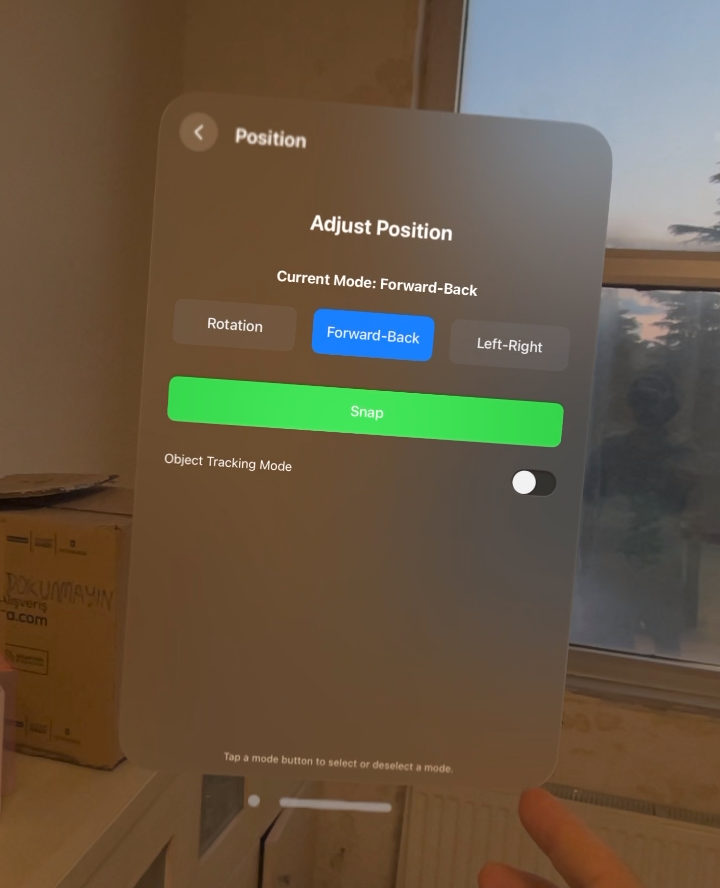
\includegraphics[width=0.47\textwidth]{repositioning_ui_new.png}
            \caption{\centering Repositioning view showing gesture-based controls and the newly added Snap and Tracking Mode buttons}
            \label{fig:ui_repositioning}
        \end{figure}


        \item \textbf{Inspection:} Inspection points are UI buttons attached to the placed object. These points activate only in the inspection view. Previously, this view included the \textit{Generate Report} button; however, in the current version, the button has been relocated to the main interaction view. (Figure \ref{fig:ui_inspection_view} shows the inspection view.)
        \begin{figure}[H]
            \centering
            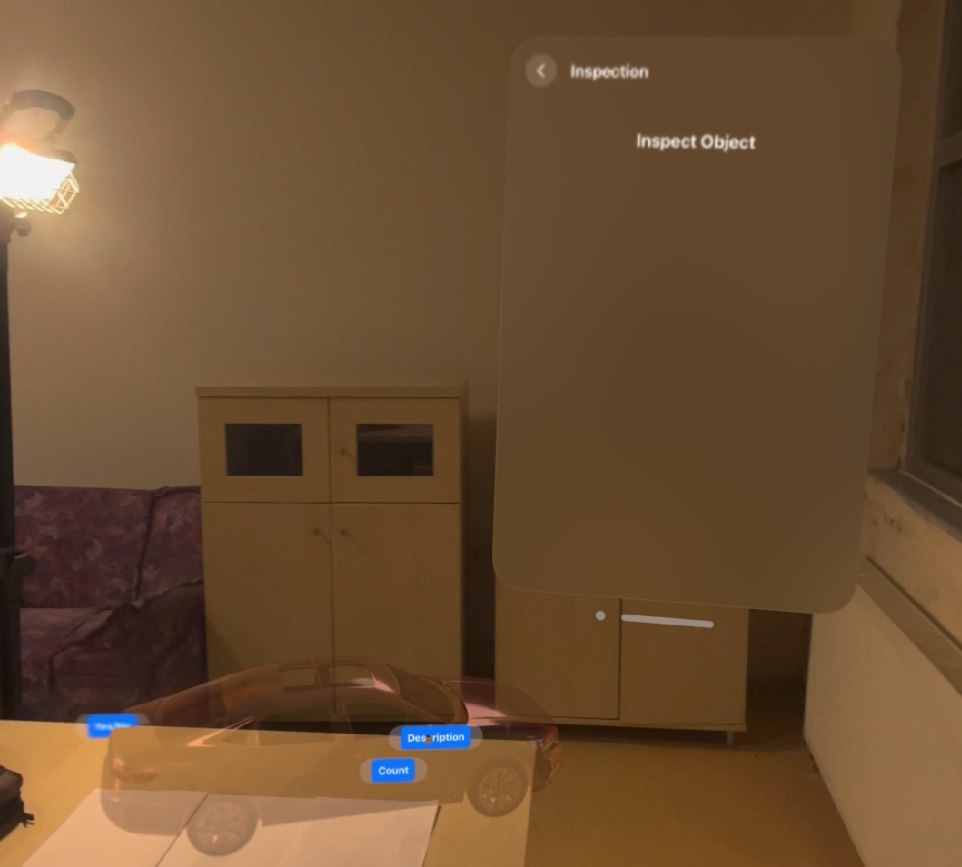
\includegraphics[width=0.6\textwidth]{inspection_view_ui.png}
            \caption{Inspection view showing active inspection points.}
            \label{fig:ui_inspection_view}
        \end{figure}

        \item \textbf{Annotation:} Introduced in the second semester, this feature allows the user to attach custom annotations directly onto the surface of the placed object. The user can tap on any point to create an annotation and enter relevant text. A search functionality is also included, enabling users to filter and locate annotations efficiently.

        \begin{figure}[H]
            \centering
            \begin{minipage}[t]{0.48\textwidth}
                \centering
                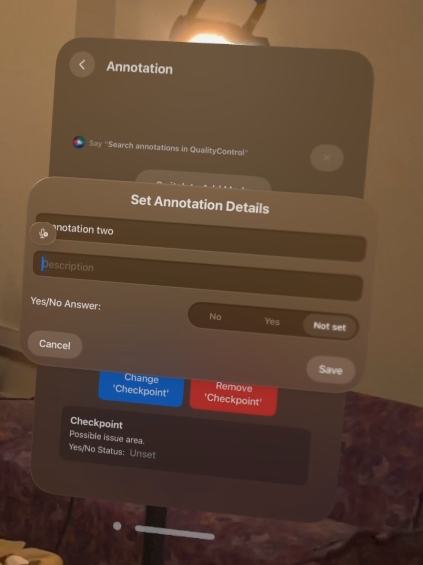
\includegraphics[width=\linewidth]{create_annotation.png}
                \caption{User creating an annotation on the object surface.}
                \label{fig:create_annotation}
            \end{minipage}
            \hfill
            \begin{minipage}[t]{0.48\textwidth}
                \centering
                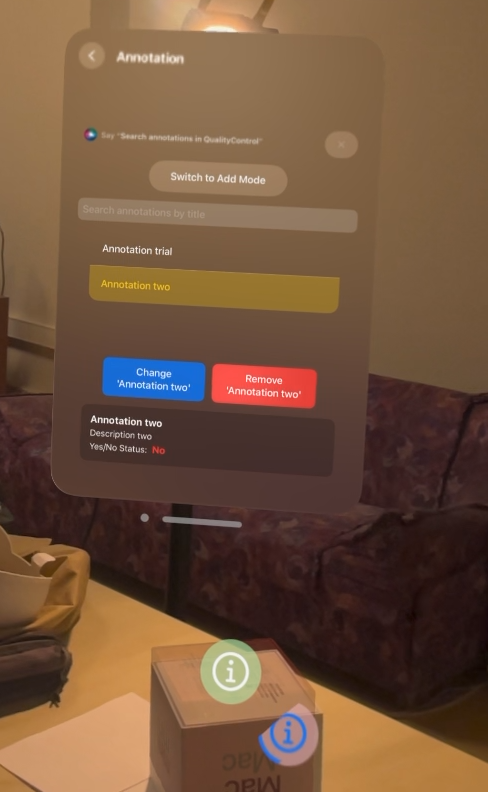
\includegraphics[width=\linewidth]{annotation_view.png}
                \caption{Annotation view showing the list of annotations attached to the object.}
                \label{fig:annotation_view}
            \end{minipage}
        \end{figure}



        \item \textbf{Generate Report:} Now placed directly within the object interaction view, this button triggers report generation without navigating away from the current screen. Upon activation, a confirmation message appears, indicating the report has been successfully generated. (Figure \ref{fig:generate_report_view} shows the confirmation message that appears after report generation.)
        \begin{figure}[H]
            \centering
            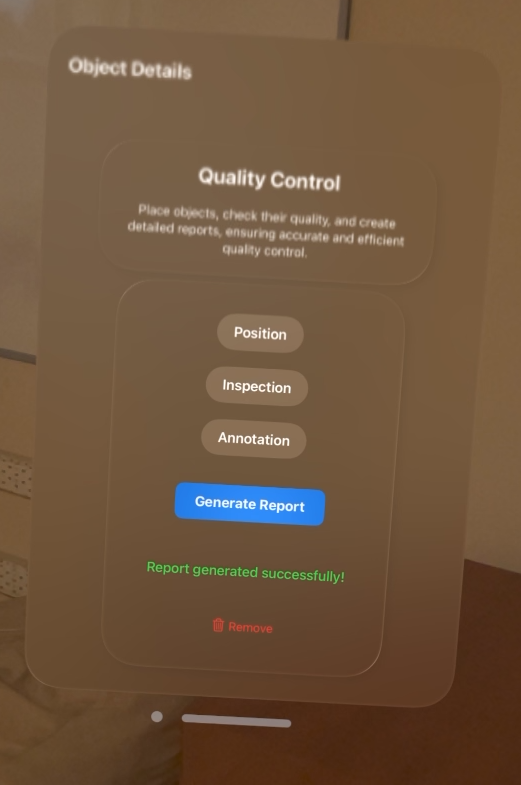
\includegraphics[width=0.4\textwidth]{generate_report_view.png}
            \caption{\centering Confirmation message indicating successful report generation.}
            \label{fig:generate_report_view}
        \end{figure}


        \item \textbf{Removal:} To remove the placed object, the user presses the remove button. A confirmation popup appears to ensure the action is intentional. (Figure \ref{fig:ui_remove_popup} shows the removal confirmation popup.)
        \begin{figure}[H]
            \centering
            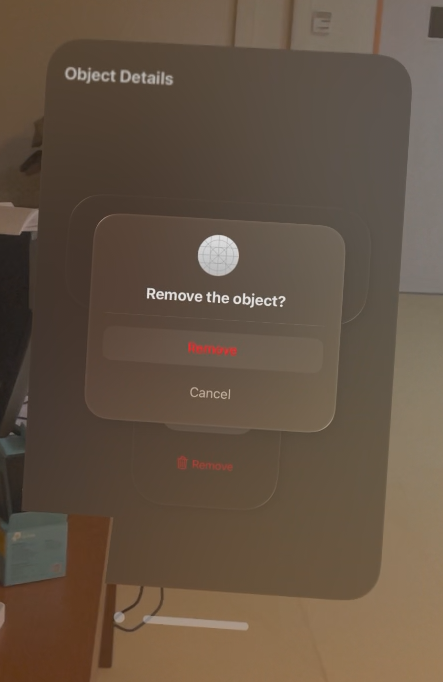
\includegraphics[width=0.4\textwidth]{remove_popup_ui.png}
            \caption{Confirmation popup for removing the placed object.}
            \label{fig:ui_remove_popup}
        \end{figure}
    \end{itemize}
\end{itemize}

\subsection{Inspection Detail View}
This component was fully implemented during the first semester and remains unchanged in the current version of the application. When an inspection point is clicked, the application navigates to the inspection detail view:
\begin{itemize}
    \item A question specific to the inspection point is displayed, which can be one of the following:
    \begin{itemize}
        \item Yes/No question.
        \item Count input.
        \item Description input.
    \end{itemize}
    \item The user provides the required input or feedback. (Figure \ref{fig:ui_inspection_detail} shows the inspection detail view.)
\end{itemize}


\begin{figure}[H]
    \centering
    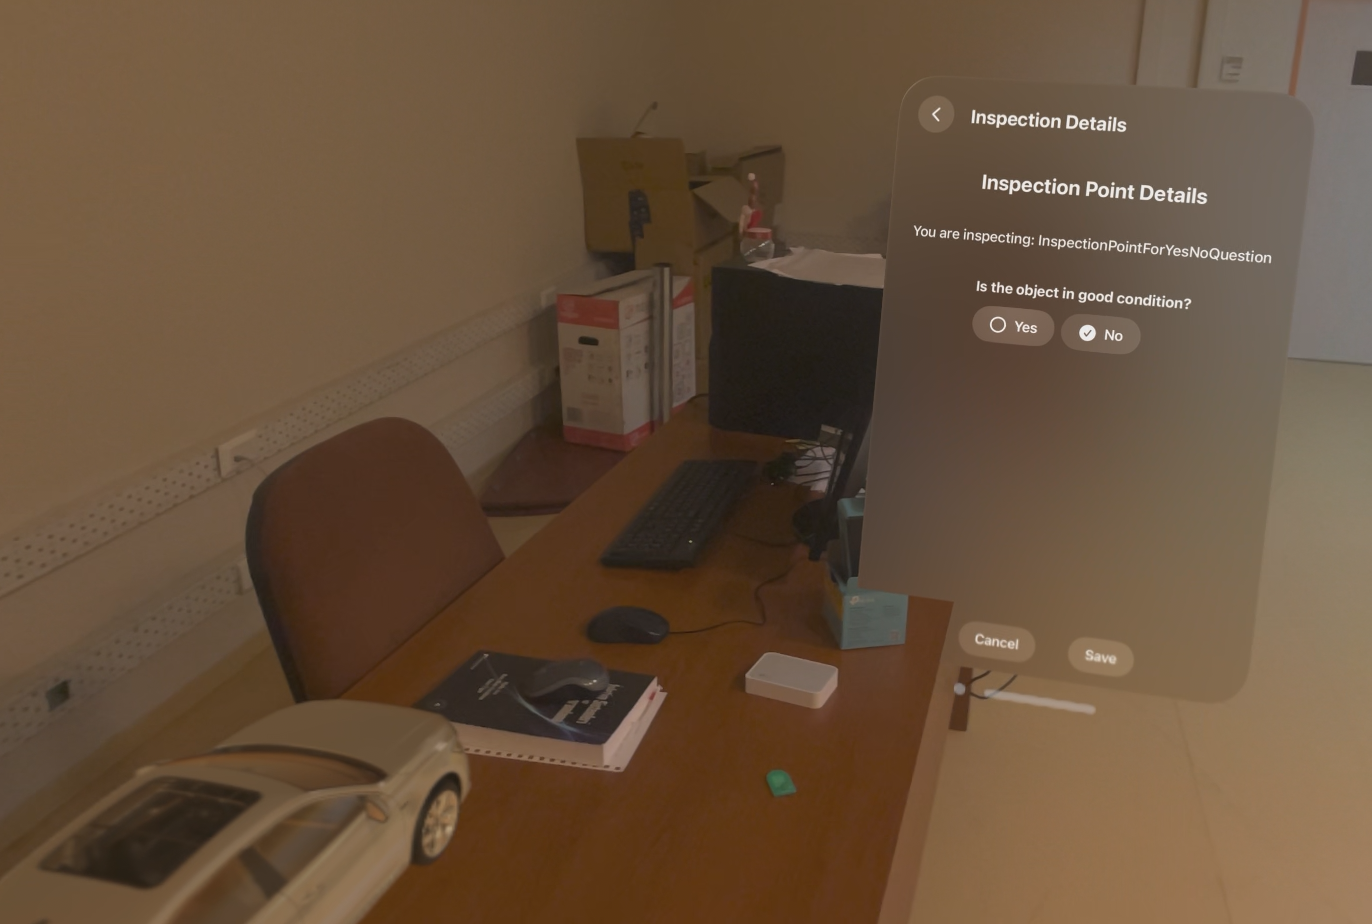
\includegraphics[width=0.8\textwidth]{inspection_detail_ui.png} % Replace with your actual file name
    \caption{Inspection detail view showing specific question types and input fields.}
    \label{fig:ui_inspection_detail}
\end{figure}

\subsection{Annotation Views}

In the second semester, an annotation system was introduced. This system uses visually responsive annotation cards that are spatially anchored to the 3D model and provide intuitive user interaction mechanisms.

\subsubsection{Annotation Card Design and Behavior}

Each annotation is represented by a UI card that is attached to a specific point on the 3D model. These cards remain anchored in space and are always oriented toward the user for readability. When the user gazes at a card, it activates a hover effect that expands the card to display more detailed information.

The expanded annotation card includes:
\begin{itemize}
    \item A \textbf{title} and \textbf{description} section.
    \item A \textbf{Yes/No} selection interface.
    
    The Yes/No state is visually encoded:
    \begin{itemize}
        \item \textbf{Green} for "Yes"
        \item \textbf{Red} for "No"
    \end{itemize}
\end{itemize}

\begin{figure}[H]
            \centering
            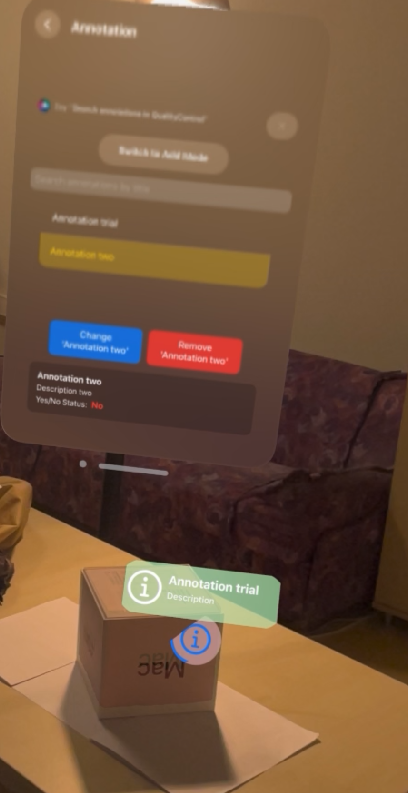
\includegraphics[width=0.4\textwidth]{annotation_card_design.png}
            \caption{Hovering annotation card design showing title, description, and Yes/No state.}
            \label{fig:annotation_card_design}
        \end{figure}

\subsubsection{Focused Annotation Mode}

There are multiple ways to activate this mode:
\begin{itemize}
    \item \textbf{Direct Focus:} The user can look at an annotation card in the AR scene and perform a pinch gesture to enter focused mode.
    \item \textbf{Menu-Based Activation:} Users can slide through a list of annotations displayed in the side menu. By looking at a list item and performing a pinch gesture, the corresponding annotation is automatically focused in the 3D view.
    \item \textbf{Search-Based Activation:} Users can search for an annotation using a built-in search bar. After locating the desired item, the user can look at it in the list and pinch to activate the focused annotation in the AR scene.
    \item \textbf{Siri Voice Search:} Users can also initiate a search by speaking to Siri. Siri automatically fills the search bar and highlights matching results in the list for pinch-based selection.
\end{itemize}

\begin{figure}[H]
            \centering
            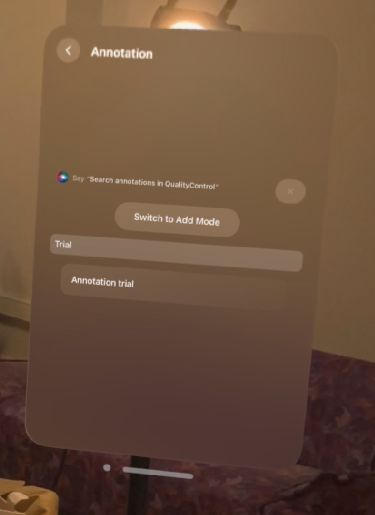
\includegraphics[width=0.4\textwidth]{annotation_search.png}
            \caption{\centering Search bar and list of annotations in the side menu. Users can search for annotations and select them to focus in the AR scene.}
            \label{fig:annotation_search}
        \end{figure}

When an annotation is focused, its card and the side menu visually changes to indicate the active state:
\begin{itemize}
    \item The annotation card turns \textbf{blue}, visually distinguishing it from other annotations in the scene.
    \item The user can then \textbf{edit} the annotation (e.g., update its title, description, or Yes/No state).
    \item The user also has the option to \textbf{remove} the focused annotation from the scene if it is no longer needed.
\end{itemize}

\begin{figure}[H]
            \centering
            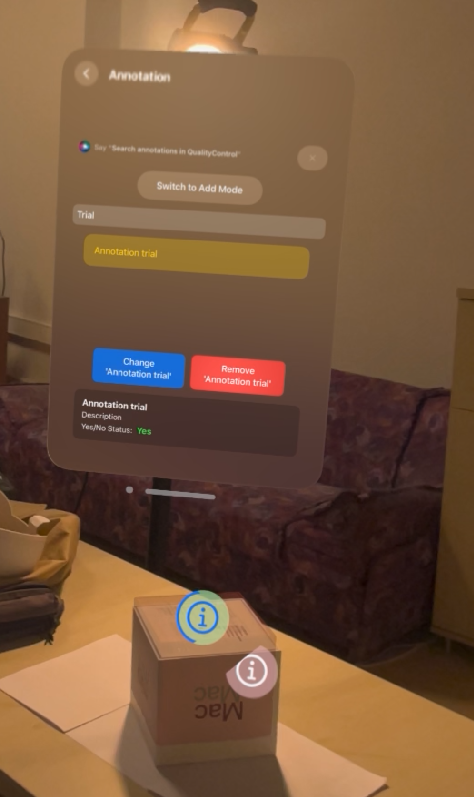
\includegraphics[width=0.4\textwidth]{annotation_focus.png}
            \caption{\centering Focused annotation card in the AR scene, showing the active state with a blue color. The user can edit or remove the annotation.}
            \label{fig:annotation_focus}
        \end{figure}




\section{Model Alignment and Object Tracking}

The system leverages ARKit’s capabilities for world tracking and plane detection to enable accurate model alignment and placement. Horizontal planes are specifically chosen to detect ground planes, ensuring precise object placement in the AR environment.

The 3D models used in the application are in the USDZ format, which is optimized for AR experiences on Apple devices.

In the second semester, we enhanced the model alignment system by integrating \textbf{object tracking} to allow more accurate and efficient placement of virtual objects in the AR environment. This feature complements ARKit’s existing plane detection and world tracking by aligning models directly to recognized real-world objects.

Additionally, to visually verify the precision of object alignment, \textbf{all 3D models were made semi-transparent and tinted red}. This visual modification enables users to inspect how accurately the virtual model overlays the physical object beneath it.


\subsection{Initial Placement}
This feature was implemented in the first semester and remains unchanged in the current version. During initial placement, the user is provided with a preview of the selected object. The preview is displayed as a greyed-out version of the object accompanied by a placement tooltip to guide the user in positioning it accurately. This feature allows the user to visually align the object with the detected ground plane before finalizing its placement, as shown in Figure \ref{fig:ui_initial_placement}.

To ensure that objects fit appropriately within the environment, size adjustments are made to the USDZ 3D models using SceneKit.

\subsection{Replacement}
This feature was introduced in the first semester and has been expanded in the second semester with additional object tracking functionality. If the user needs to reposition an already placed object, they can do so in the position mode of the application. In this mode:
\begin{itemize}
    \item The user can perform object rotation, as well as left/right and forward/backward movements.
    \item These adjustments are enabled only when the position mode is activated in the position view.
    \item Pinch and drag gestures (thumb and index finger) are used to perform these actions, as shown in Figure \ref{fig:ui_repositioning}.
    \item Two new buttons were added:
    \begin{itemize}
        \item \textbf{Snap Button:} Aligns the virtual model with the most recent object tracking data from ARKit.
        \item \textbf{Object Tracking Mode Toggle:} Continuously updates the model’s position and orientation using live tracking data when enabled.
    \end{itemize}
\end{itemize}

\subsection{Object Tracking}
To enable object tracking, each tracked model is paired with a reference object file in addition to its USDZ representation. These reference object files were generated using Xcode’s machine learning tool, which extracts object recognition data from the USDZ models.

We used iPhone Pro models equipped with LiDAR sensors to improve the accuracy of 3D reconstruction. This provided better depth data and enabled the creation of more reliable reference objects.

Textured and visually distinct objects were intentionally chosen to support more robust detection and tracking performance.

% Explanation about inspection will go here.
\section{Inspection}

All inspection operations, including providing input to inspection points and viewing inspection points, occur exclusively within the \textbf{Inspection View}. If the application is not in the \textbf{Inspection View}, all inspection points are removed from the interface. When the user navigates back to the \textbf{Inspection View}, the inspection points are dynamically regenerated (as shown in Figure \ref{fig:ui_inspection_view}).

To prevent user confusion or potential issues (e.g., uncertainty about whether data is saved), all inspection points are also removed when the application navigates to the \textbf{Inspection Detail View}. This design decision ensures reliability and eliminates bugs arising from unclear save states or interactions (as shown in Figure \ref{fig:ui_inspection_detail}).

The inspection system was fully implemented in the first semester and remains unchanged in the current version, with the exception of the removal of the \textbf{Generate Report} button from the \textbf{Inspection View}. Report generation has been moved to the object interaction view.

\subsection{Inspection Points}
For each inspection point on the placed model, a UI button is displayed (as shown in Figure \ref{fig:ui_inspection_view}). These buttons are dynamically positioned based on the specific locations of the inspection points on the model. When the user clicks an inspection point button, the application navigates to the \textbf{Inspection Detail View}, where the selected inspection point can be reviewed and updated.

\subsection{Inspection Detail View}
In the \textbf{Inspection Detail View}, users can perform inspections on the selected point. The system supports three types of inspections:
\begin{itemize}
    \item \textbf{Yes/No:} A binary choice indicating whether the inspection criteria have been met, as shown in Figure \ref{fig:ui_inspection_detail}.
    \item \textbf{Count:} Allows the user to input the quantity of specific elements related to the inspection point.
    \item \textbf{Description:} Provides a text field for the user to enter detailed notes or comments about the inspection point.
\end{itemize}

% Explanation about the Annotation system will go here.

% Explanation about generating reports will go here.
\section{Report Generation}

The report generation functionality in this system is powered by the third-party C library \textbf{libxlsxwriter}, which facilitates the creation of Excel files. This feature enables users to export inspection reports, which are saved directly to the Apple Vision Pro's local directory for easy access. While the initial implementation in the first semester focused on exporting object and inspection point data, this semester the functionality was extended to include annotations in the report.

\subsection{Implementation Overview}
Each report file is named dynamically based on the object being inspected and a unique identifier to avoid conflicts.

\subsection{Report Content}
The generated report contains the following key information:
\begin{itemize}
    \item \textbf{Object Details:} The name, width, height, and depth of the inspected object are recorded in the report.
    \item \textbf{Inspection Points:} Each inspection point associated with the object is detailed in the report. For every inspection point, the following attributes are included:
    \begin{itemize}
        \item \textbf{Name:} The identifier of the inspection point.
        \item \textbf{Depending on The Type of Inspection:}
        \begin{itemize}
            \item \textbf{Count:} The quantity associated with the inspection point, if applicable.
            \item \textbf{Description:} Detailed notes or observations provided by the user.
            \item \textbf{Is Correct:} A binary value (Yes/No) indicating whether the inspection point meets the desired criteria.
        \end{itemize}
    \end{itemize}
    \item \textbf{Annotations} \textit{(Second Semester):} Annotation cards added to the object in the AR scene are also included in the report. For each annotation:
    \begin{itemize}
        \item \textbf{Title:} The title of the annotation.
        \item \textbf{Description:} Textual content describing the annotation.
        \item \textbf{Yes/No State:} Whether the annotation is marked "Yes" or "No."
    \end{itemize}
\end{itemize}

An example of the generated Excel report, including both inspection and annotation data, is shown in Figure \ref{fig:example_excel}.

\begin{figure}[H]
    \centering
    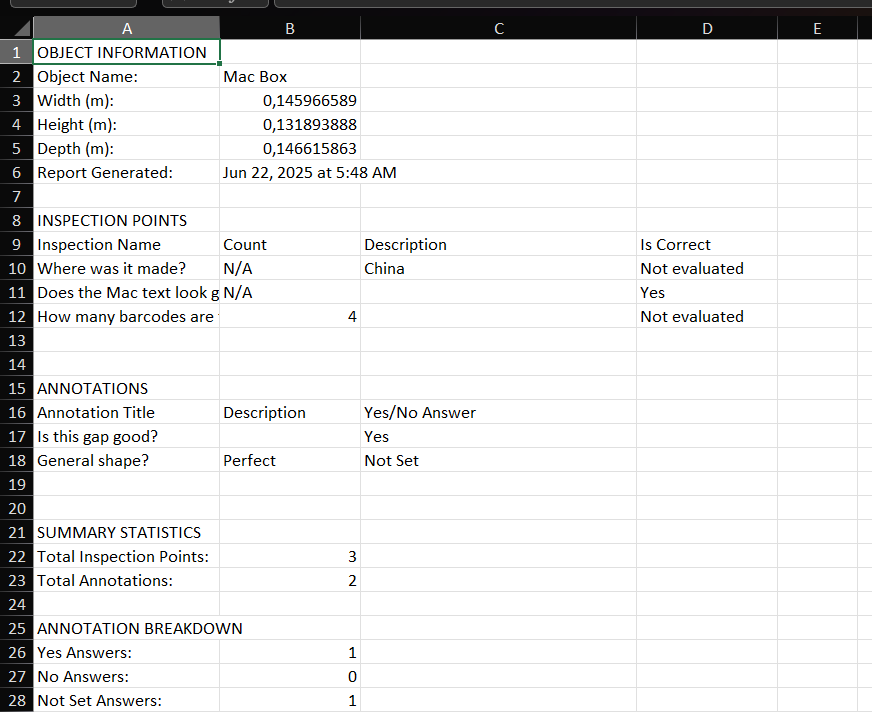
\includegraphics[width=0.8\textwidth]{example_excel.png} % Replace with your actual file name
    \caption{Example Excel report generated by the application, including inspection and annotation data.}
    \label{fig:example_excel}
\end{figure}
% \end{itemize}

% An example of the generated Excel report is shown in Figure \ref{fig:example_excel}.
% \begin{figure}[h!]
%     \centering
%     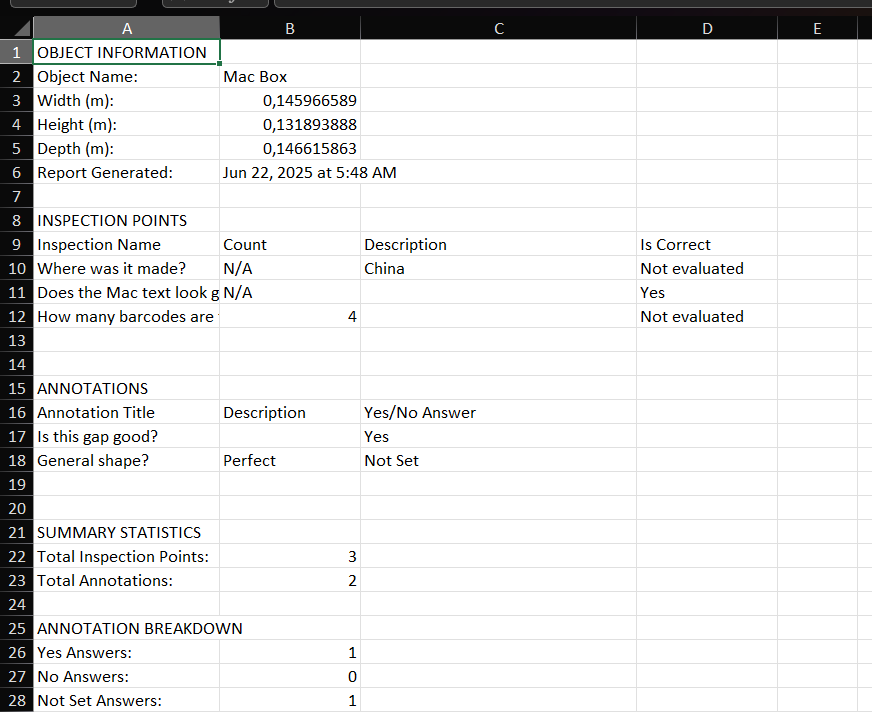
\includegraphics[width=0.8\textwidth]{example_excel.png} % Replace with your actual file name
%     \caption{Example Excel report generated by the application.}
%     \label{fig:example_excel}
% \end{figure}

\subsection{Integration with Apple Vision Pro}
The reports are stored locally on the Apple Vision Pro device, allowing users to access them conveniently through the file system. This integration ensures compatibility with the Vision Pro environment and leverages the device's capabilities for efficient data handling.

By using \textbf{libxlsxwriter}, the system provides a robust and efficient way to generate and manage detailed Excel reports, enhancing the overall functionality and usability of the quality control application.



\section{Use Case Diagram}
The use case diagram below illustrates the interaction between the user and the primary functionalities of the system.

\begin{landscape}
\begin{center}
    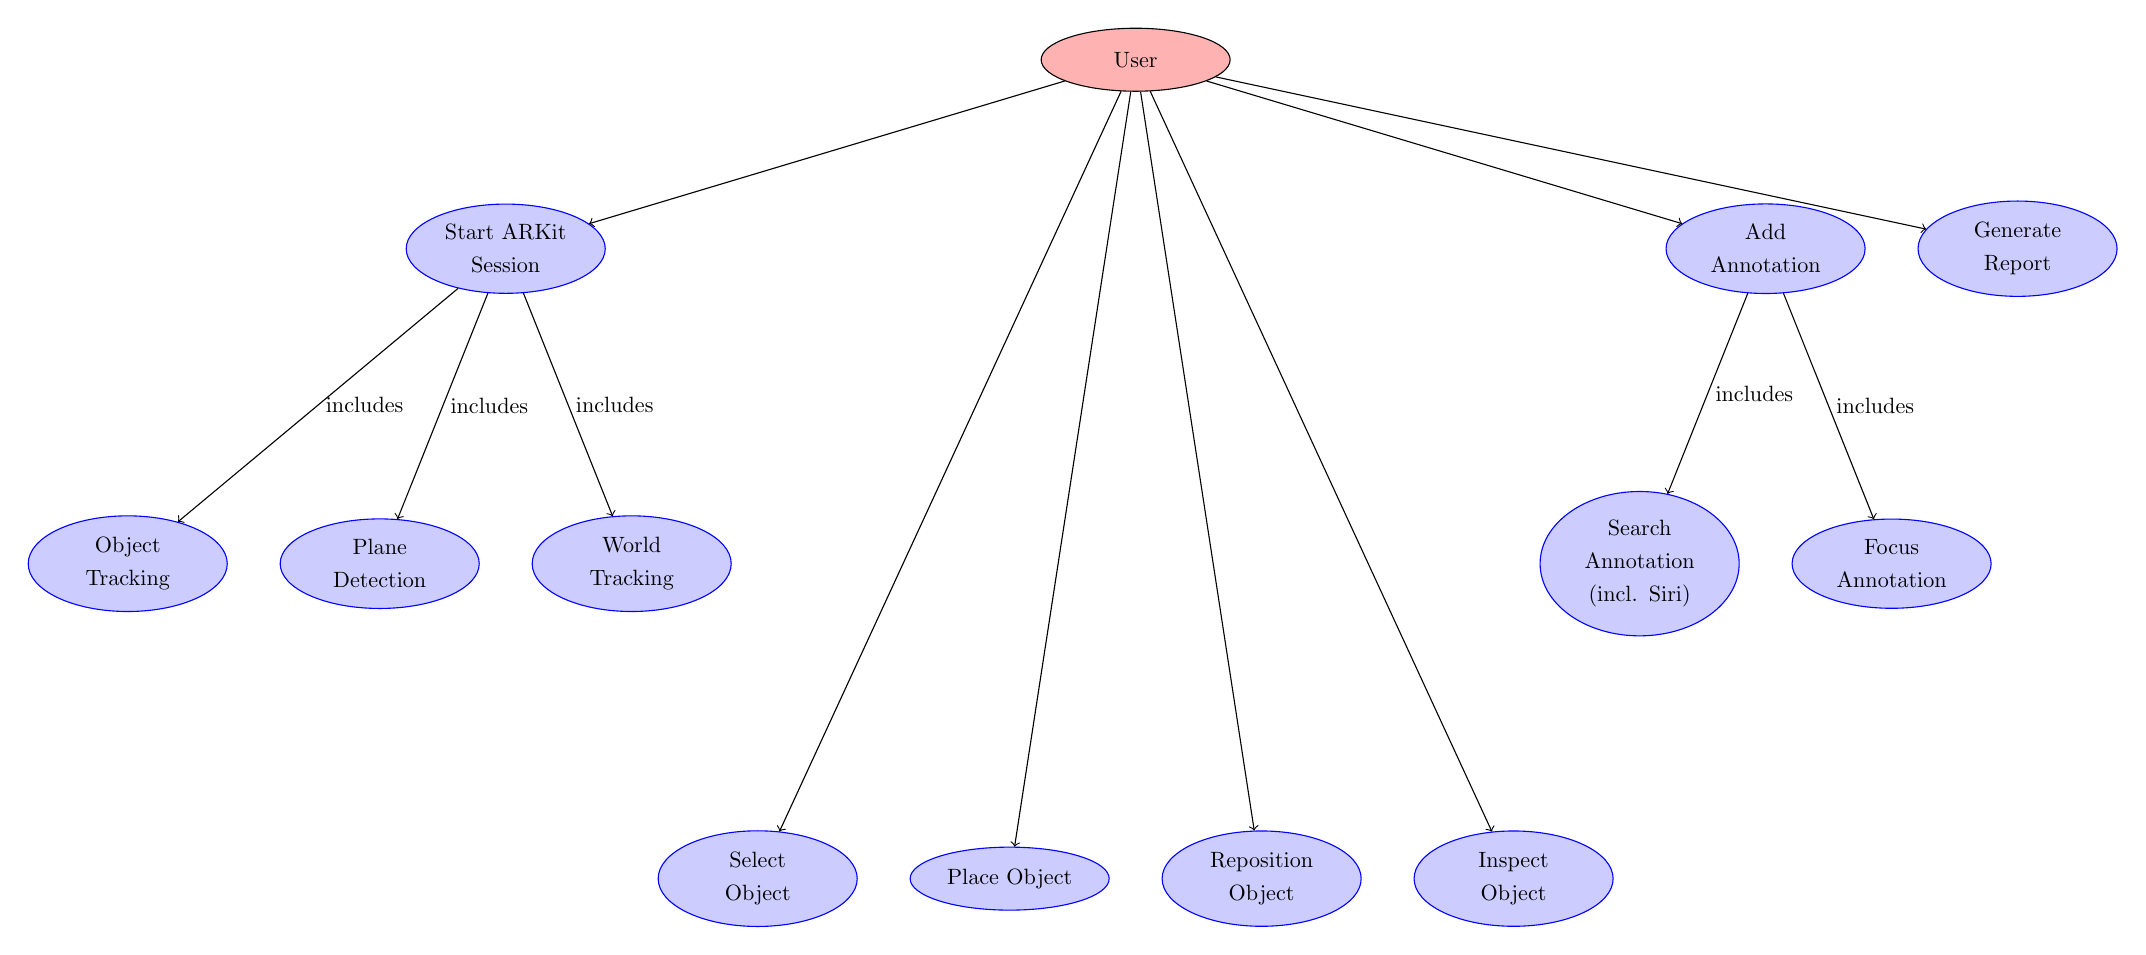
\begin{tikzpicture}[node distance=3cm, scale=0.8, transform shape]

        % Actor
        \node (user) [actor] {User};

        % Use cases
        \node (start) [usecase, below of=user, xshift=-10cm] {Start ARKit Session};
        \node (select) [usecase, below of=user, yshift=-10cm, xshift=-6cm] {Select Object};
        \node (place) [usecase, below of=user, yshift=-10cm, xshift=-2cm] {Place Object};
        \node (reposition) [usecase, below of=user, yshift=-10cm, xshift=2cm] {Reposition Object};
        \node (inspect) [usecase, below of=user, yshift=-10cm, xshift=6cm] {Inspect Object};
        \node (addanno) [usecase, below of=user, xshift=10cm] {Add Annotation};
        \node (report) [usecase, below of=user, xshift=14cm] {Generate Report};

         % Sub-use cases for ARKit session
        \node (tracking) [usecase, below of=start, xshift=-6cm, yshift=-2cm] {Object Tracking};
        \node (plane) [usecase, below of=start, xshift=-2cm, yshift=-2cm] {Plane Detection};
        \node (world) [usecase, below of=start, xshift=2cm, yshift=-2cm] {World Tracking};

        % Sub-use cases for Annotation
        \node (search) [usecase, below of=addanno, xshift=-2cm, yshift=-2cm] {Search Annotation (incl. Siri)};
        \node (focus) [usecase, below of=addanno, xshift=2cm, yshift=-2cm] {Focus Annotation};

        % Connections between actor and use cases
        \draw [->] (user) -- (start);
        \draw [->] (user) -- (select);
        \draw [->] (user) -- (place);
        \draw [->] (user) -- (reposition);
        \draw [->] (user) -- (inspect);
        \draw [->] (user) -- (addanno);
        \draw [->] (user) -- (report);
        
        % Relationships between use cases
        \draw [->] (start) -- node[midway, right] {includes} (tracking);
        \draw [->] (start) -- node[midway, right] {includes} (plane);
        \draw [->] (start) -- node[midway, right] {includes} (world);

         \draw [->] (addanno) -- node[midway, right] {includes} (search);
    \draw [->] (addanno) -- node[midway, right] {includes} (focus);

    \end{tikzpicture}
\end{center}
\end{landscape}


\chapter{Conclusion and Results}

This chapter presents the evaluation of the quality control system based on the redefined success criteria for the second phase: \textbf{tracking stability}, \textbf{annotation accuracy}, and \textbf{inspection completion time}. The following sections detail how the system performed in each area, reflecting the impact of the new custom annotation and object tracking features.

\section{Tracking Stability}

Tracking stability was evaluated by measuring the positional variance between the corners of the real object (a Mac Mini box) and the corresponding corners of the virtual model, after snapping the model into place in AR. For this test, the real object was positioned in a fixed, predefined location, and the eight corner points of the Mac Mini box were chosen as reference locations for measurement. Once the virtual model was aligned with the real object, the distances between each actual corner and the corresponding model corner were measured while wearing the device.

Figure~\ref{fig:tracking_measurement} illustrates the setup for these measurements, showing both the spatial arrangement of corner points and the viewpoint used for evaluation. In this test, the observer looked at the object from an upper front corner (see Figure~\ref{fig:tracking_measurement}, bottom right), which produced relatively consistent results on the front and top faces. However, variances were noticeably larger at the backside corners, likely due to sensor limitations and occlusion effects from this viewing angle.

The measurement results are presented in Table~\ref{tab:tracking_variance}. The right side variances were: 0.5, 0.4, 0.5, and 0.4 cm. The left side variances were: 0.9, 0.2, 0.7, and 1.0 cm. The **average variance** across all measured points was \textbf{0.575 cm} (5.75 mm), which is close to the target of 5 mm maximum variance.

\begin{table}[h!]
    \centering
    \caption{Measured positional variances (in cm) for each corner of the Mac Mini box}
    \label{tab:tracking_variance}
    \begin{tabular}{|c|c|c|c|c|c|c|c|c|}
        \hline
        \textbf{Corner} & 1 (R) & 2 (R) & 3 (R) & 4 (R) & 5 (L) & 6 (L) & 7 (L) & 8 (L) \\
        \hline
        \textbf{Variance (cm)} & 0.5 & 0.4 & 0.5 & 0.4 & 0.9 & 0.2 & 0.7 & 1.0 \\
        \hline
    \end{tabular}
\end{table}


\noindent
\textbf{Average variance:} 0.575 cm

\vspace{1em}

\noindent
\textbf{Remarks:}
The model used for these measurements was generated using an iPhone Pro's object capture feature (LiDAR-based). While generally reliable, this model exhibits some minor inaccuracies, particularly due to the small size of the scanned object (13\,cm $\times$ 13\,cm), which increases sensitivity to reconstruction errors compared to larger objects. Additionally, certain areas lack detailed texture, further impacting model accuracy. Although LiDAR sensors help address some of these challenges, their effectiveness is limited in regions with poor or missing surface texture. As a result, a portion of the observed tracking errors can be attributed to these model imperfections rather than to the AR tracking system itself.

\begin{figure}[h!]
    \centering
    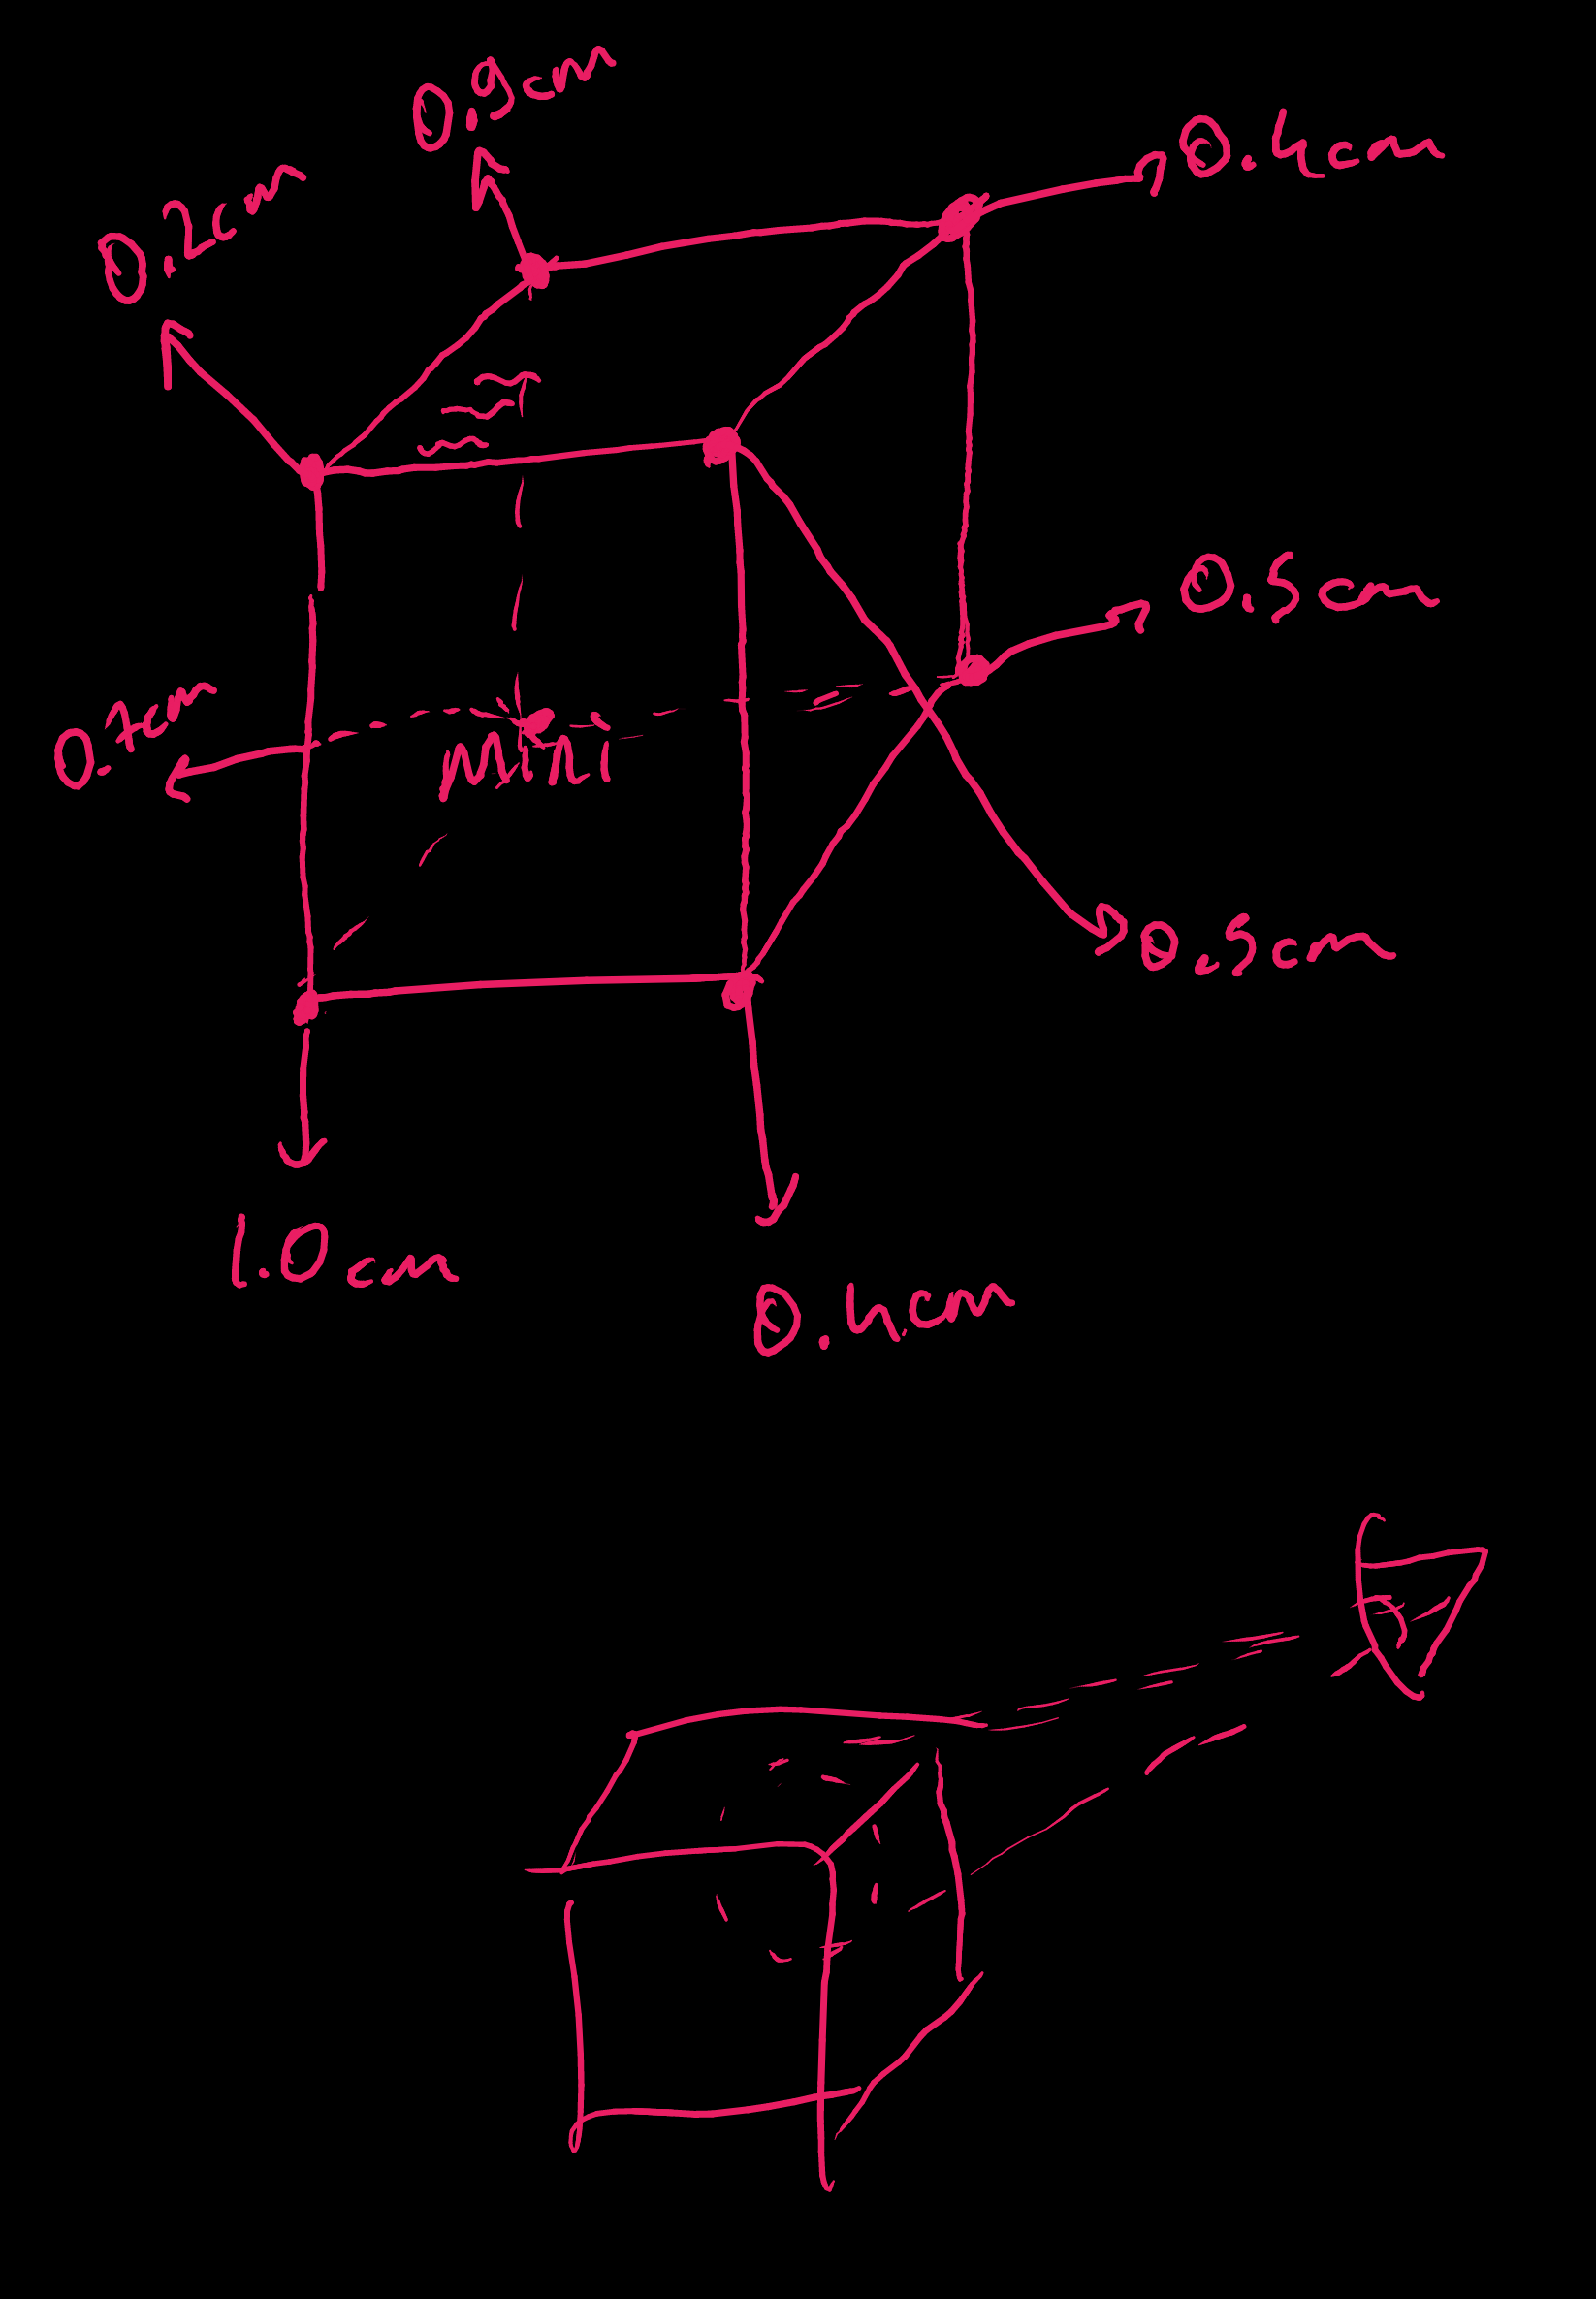
\includegraphics[width=0.4\textwidth]{tracking_stability.png}
    \caption{Setup for tracking stability measurements. Corner variances are shown at each location. The observer's viewpoint during measurement is depicted at bottom right.}
    \label{fig:tracking_measurement}
\end{figure}
\section{Annotation Accuracy}

To assess annotation search efficiency and user experience, we placed 100 numbered annotation points on the test model. Users were prompted with a random annotation number (0–100) and asked to locate it using three different input methods: Siri (voice search), virtual keyboard text input, and keyboard text-to-speech. For each attempt, the time required for initiating the search (input), selecting the annotation from the filtered list, and completing the entire process was recorded.

Table~\ref{tab:annotation_accuracy_breakdown} presents the results for each method, separating the search/input and list selection stages where available.

\begin{table}[h!]
    \centering
    \caption{Annotation search times (in seconds) by input method and stage}
    \label{tab:annotation_accuracy_breakdown}
    \begin{tabular}{|l|c|c|c|}
        \hline
        \textbf{Method} & \textbf{Search/Input} & \textbf{List Selection} & \textbf{Overall Time} \\
        \hline
        Siri & 8 & 7 & 15 \\
        Siri & 6 & 5 & 11 \\
        Siri & 7 & 3 & 10 \\
        Siri & 5 & 2 & 7 \\
        Siri & 5 & 2 & 7 \\
        Siri & 8 & 3 & 11 \\
        \hline
        \textbf{Avg. Siri} & 6.5 & 3.7 & 10.2 \\
        \hline
        Keyboard Text & -- & -- & 6 \\
        Keyboard Text & -- & -- & 3 \\
        \hline
        \textbf{Avg. Keyboard Text} & -- & -- & 4.5 \\
        \hline
        Text-to-Speech & 6 & 2 & 8 \\
        Text-to-Speech & 3 & 1 & 4 \\
        Text-to-Speech & 4 & 1 & 5 \\
        \hline
        \textbf{Avg. Text-to-Speech} & 4.3 & 1.3 & 5.7 \\
        \hline
    \end{tabular}
\end{table}

\noindent
\textbf{Analysis:} For the Siri method, the workflow involved activating Siri (e.g., “Hey Siri, find annotations in quality control”), followed by list filtering and selecting the target annotation. The Siri system’s response time was the largest contributor to total duration, often taking between 5–8 seconds before the user could proceed to list selection. Selection from the filtered list was consistently fast (1–7 seconds). 

With the virtual keyboard text input, the entire process was generally faster (3–6 seconds), but still hindered by the relative slowness and awkwardness of typing on a virtual keyboard within Vision Pro. The text-to-speech method, in contrast, enabled the fastest initiation (3–6 seconds for search), and users consistently completed the process within 4–8 seconds overall.

Notably, for all methods, once the annotation list was filtered, users were able to select and visually identify the annotation on the AR model in well under 3 seconds—demonstrating that the annotation system itself is intuitive and efficient. Most delays arose from the time required for input or system dialog, especially in the Siri scenario.

\vspace{1em}
\noindent
\textbf{Conclusion:} Although the end-to-end annotation search time did not always meet the strict 3-second target—mainly due to input method delays—the process was generally close, especially for text and speech-based approaches. Further optimization of input methods, particularly Siri response latency and keyboard usability, would enable more consistent achievement of the target and further streamline the annotation workflow for industrial use.


\section{Inspection Completion Time}

Directly comparing inspection completion times between our system and a tablet-based solution was challenging due to limited access to comparable resources and scenarios. Since we could not arrange a fully matched test using the same users, objects, and inspection complexity, we relied on publicly available demonstration videos.

Specifically, we analyzed a YouTube video in which a user performed a sequence of inspection tasks on a tablet-based AR quality control application. The workflow in the video included snapping a virtual object to a real object, creating six annotation points, modifying and deleting annotations, and finally adding a description annotation. The entire process took \textbf{60 seconds}.

We replicated this workflow as closely as possible on our Vision Pro system, following the same order and number of operations. In our trial, the total completion time was \textbf{76 seconds}.

\begin{table}[h!]
    \centering
    \caption{Inspection completion time comparison}
    \label{tab:inspection_completion_time}
    \begin{tabular}{|l|c|c|c|}
        \hline
        \textbf{Task} & \textbf{Tablet (s)} & \textbf{Vision Pro (s)} & \textbf{Relative to Tablet (\%)} \\
        \hline
        Inspection scenario & 60 & 76 & 79 \\
        \hline
    \end{tabular}
\end{table}


\vspace{1em}
\noindent
\textbf{Interpretation:} Our goal was to achieve at least 80\% of the inspection speed of a tablet-based solution in a comparable scenario. While our result (79\%) is slightly below this threshold, the test conditions were not perfectly matched, and some variance is expected due to differences in model geometry, user familiarity, and interface details. Nevertheless, the Vision Pro system demonstrated comparable inspection workflow efficiency, with completion times close to those achieved on established tablet-based systems.


\section{Summary of Results}

The developed system demonstrated strong tracking stability (average 5.75~mm variance), efficient annotation search (with users typically locating annotations in a few seconds), and inspection completion time close to tablet-based solutions (76~s vs.\ 60~s). While some results were just below target benchmarks, overall performance is robust and the new features introduced in this phase provide clear improvements for industrial quality control tasks.

\section{Conclusion}

This thesis described the design, implementation, and evaluation of an augmented reality (AR)-based quality control system for the Apple Vision Pro. Building on an initial version, the second phase focused on enabling precise object tracking, dynamic (user-defined) annotations, and enhanced reporting, leveraging the device’s advanced spatial and interaction capabilities.

\subsection{Summary of Achievements}
The developed system now supports:
\begin{itemize}
    \item \textbf{Robust Tracking:} Accurate and stable alignment between virtual models and real-world objects, with average tracking variance close to industrial standards.
    \item \textbf{Dynamic Annotations:} Users can create and manage custom annotation points, enabling more flexible and realistic inspection scenarios.
    \item \textbf{Advanced Reporting:} Inspection results—including dynamic annotations—can be exported for further analysis.
    \item \textbf{Competitive Performance:} Annotation search and inspection completion times are close to tablet-based benchmarks, validating the system’s practicality for real-world quality control.
\end{itemize}

\subsection{Challenges and Limitations}
Despite these advances, some challenges remain:
\begin{itemize}
    \item \textbf{Input Modality Latency:} Voice and keyboard inputs, especially via Siri and virtual keyboards, still limit search speed in some workflows.
    \item \textbf{3D Model Quality:} Minor inaccuracies in captured models can affect ultimate tracking precision.
    \item \textbf{Camera Inaccessibility:} Limited access to raw camera data on Vision Pro prevents the use of custom computer vision algorithms and makes it impossible to attach photos directly to annotations.
    \item \textbf{Swift and Apple Development Constraints:} The development environment restricts certain low-level customizations, limiting the integration of fully custom algorithms and advanced features.
\end{itemize}


\subsection{Future Work}
To further advance the system, the following directions are proposed:
\begin{itemize}
    \item \textbf{Improved Input Methods:} Optimize and streamline voice and text input for annotation search and inspection, possibly leveraging more advanced natural language processing and multi-modal interaction.
    \item \textbf{Automated Inspection Points:} Integrate computer vision and machine learning techniques to automatically generate and recommend inspection points based on object geometry and historical inspection data.
    \item \textbf{Photo and Media Annotations:} Enable attaching photos, videos, or additional media to annotation points—pending camera access, which typically requires an Apple enterprise development account.
    \item \textbf{User Experience Evaluation:} Conduct extensive user studies in real industrial environments to gather feedback and guide further refinement of workflows and interface design.
\end{itemize}


\subsection{Final Remarks}
This work demonstrates the potential of next-generation AR headsets for practical quality control. The Apple Vision Pro platform enables more dynamic, immersive, and precise inspection workflows, providing a strong foundation for future industrial AR solutions.




% DON'T INPUT FILES AFTER HERE
\begin{outertitles}
\clearpage
\setlength{\emergencystretch}{1em}
\printbibliography
\addtocontents{toc}{\protect\vspace{18pt}}
% \addcontentsline{toc}{chapter}{Bibliography}
%% If you don't want a CV or appendices add a % at the beginning of the relevant line
\chapter*{Contributions}
\addcontentsline{toc}{chapter}{Contributions}

This project was a collaborative effort between the two authors, BİLAL GÖKÇE and MELİKE SEYİTOĞLU. Below is a breakdown of the key responsibilities and contributions of each team member:

\begin{itemize}
    \item \textbf{BİLAL GÖKÇE:}
    \begin{itemize}
        \item UI/UX design, including main application models and views.
        \item Feature integration across all major modules of the application.
        \item Testing and debugging of the application.
    \end{itemize}
    \item \textbf{MELİKE SEYİTOĞLU:}
    \begin{itemize}
        \item Implementation of the custom annotation UI.
        \item Development of object tracking functionality.
        \item Addition of LLM-based annotation search feature.
        \item Testing and debugging of the application.
    \end{itemize}
\end{itemize}

The success of the project was made possible through close collaboration and regular communication between the team members.

\chapter*{References}
\addcontentsline{toc}{chapter}{References}

\begin{enumerate}
    \item Apple VisionOS Developer Site (Also For Template Projects): \url{https://developer.apple.com/visionos/}
    \item Apple Vision Pro Documentation: \url{https://developer.apple.com/documentation/visionos}
    \item SupAR Website (iPad App): \url{https://supar.eu/}
    \item A C Library For Creating Excel XLSX Files: \url{https://github.com/jmcnamara/libxlsxwriter}
    \item Unity Apple Vision Pro Development Site: \url{https://unity.com/campaign/spatial}
    \item Transforming RealityKit Entities with Gestures – Apple Developer Documentation: \url{https://developer.apple.com/documentation/realitykit/transforming-realitykit-entities-with-gestures}
    \item 3-Sweep: Extracting Editable Objects from a Single Photo, ACM Transactions on Graphics, 32(6), November 2013.\\
        DOI: \url{10.1145/2508363.2508378}
    \item Scanning Objects Using Object Capture – Apple Developer Documentation: \url{https://developer.apple.com/documentation/realitykit/scanning-objects-using-object-capture}
    \item SiriKit – Apple Developer Documentation: \url{https://developer.apple.com/documentation/sirikit/}
\end{enumerate}

\appendix
\chapter{Appendix}

\section{Annotation Accuracy Test Setup}
Figure~\ref{fig:annot_test_setup} shows the experimental setup for the annotation accuracy test. Numbered annotation points were placed on the model, and users attempted to locate specific annotations using different input methods (Siri, virtual keyboard, and text-to-speech).

\begin{figure}[h!]
    \centering
    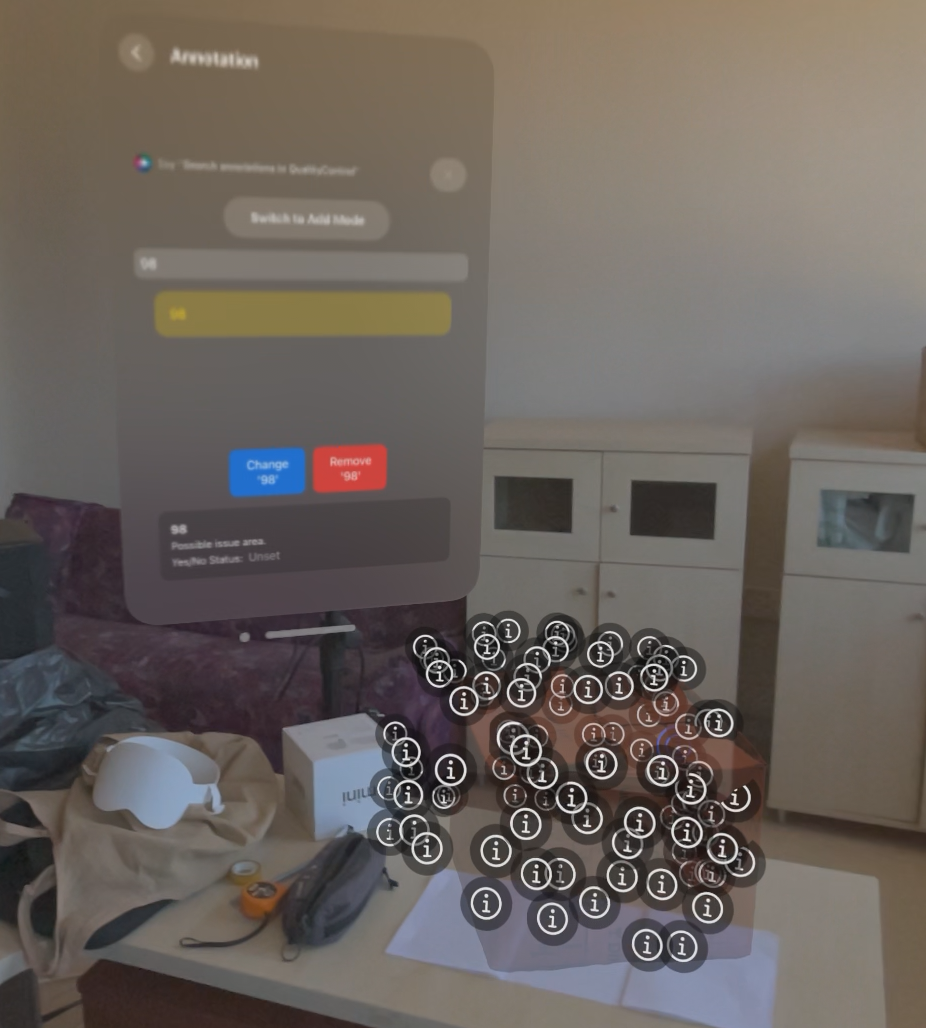
\includegraphics[width=0.7\textwidth]{../Imgs/100_annotations.png}
    \caption{Setup for annotation accuracy test: 100 annotations on a model with search performed using Siri, keyboard, and text-to-speech.}
    \label{fig:annot_test_setup}
\end{figure}


\end{outertitles}
\end{document}